\chapter{Index Analysis of the MNA}

der ane satz do + proof hopefully

seite 22 kap 7 netw top and dae ind for rlc - modelling and discretization circ prob

In the linear case, the capacitances, inductances and resistances are symmetrical positive definite (We consider them as matrices in this case). In the nonlinear case ... . Then it is called an RLC network.

In our further analysis we will only consider such RLC networks.

\subsection{General Index analysis}

Assuming the system only contains linear elements or is linearized at an operating point in order to investigate the system behaviour then the corresponding network equation represent a DAE with constant coefficients \ref{DAE-const-coeff}. Ww will denote $x=(u i_L i_V)^\top$.

\begin{itemize}
	\item \textbf{ODE-case}: \newline
	The matrix $B$ is regular in \ref{DAE-const-coeff}. This is the case if
	\begin{figure}[H]
		\centering
		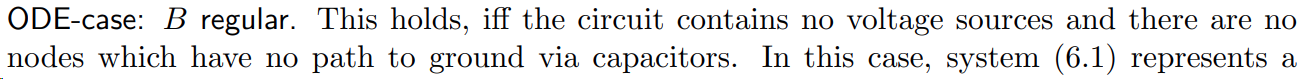
\includegraphics[width=0.7\linewidth]{screenshot006}
		\caption{}
		\label{fig:screenshot006}
	\end{figure}
	, then the system represents  alinear-implicit system of ODEs and can be transformed into the explicit ODE sytstem
	\begin{displaymath}
		\dot{x}=B^{-1}(-Ax+f(t))
	\end{displaymath}
	
	\item \textbf{DAE-case}:
	The matrix $B$ is singular in \ref{DAE-const-coeff}. In the following we will assume $D$ to be regular. Multiplying with $D^{-1}$ from the left side produces
	\newline
	nevermind thats the same as we did in the \ref{DAE-const-coeff} chapter. - reference to that an explain in these terms. - page 20
\end{itemize}

\subsection{Topological Conditions}
For this we consider RLC networks with independant voltage and current sources (\textbf{what does that mean?}). To obtain the perturbation index of the MNA we perturb the right-hand side of  
\newline reference to Tischendorf

\cite{Tischendorf2004Topological}